\chapter{Concluding Remarks}

In this work, we introduced a strategy to help to identify rules to avoid useless mutants, i.e., equivalent and duplicated mutants. 
As input, we pass a set of programs. 
For each program \textit{P}, the strategy also needs a passing test suite and a set of mutants derived from \textit{P}. 
As output, our strategy yields a set of useless mutants candidates. 
To evaluate the strategy, we used 4,999 mutants. 
The strategy classified 963 as equivalent and 1,332 as duplicated. 
By carefully analyzing this output, we derived \NumberOfNewHeuristics new rules. 

Because we derived the rules by using artificial and small Java programs, we decided to implement a subset of our rules in the \mujava{} mutation tool to check whether our rules can identify useless mutants in industrial-scale projects. 
By using well-known open-source projects, we could avoid the generation of almost 13\% of useless mutants, on average. 
This result is relatively low when compared to related work, but it is promising because, instead of generating and checking whether the mutants are indeed useless, we do not generate the useless mutants at all. 
In addition, we can derive and implement more rules in case we set our strategy to use more complex programs.

To understand the overhead brought by our technique, we executed the new \mujava{} version embedded with \NumberOfImplementedHeuristics rules in the same industrial-scale systems and compared against the original \mujava{} version.
In spite of the additional overhead, the new \mujava{} version had a payoff higher than 12\% for all projects and reached almost 20\% in two projects. 

Our technique does not eliminate other solutions that detect mutants after their generation. 
Therefore we believe that combining two or more techniques may increase the adoption of mutation testing by the industry.

%To derive more rules, as future work we intend to set our strategy to use different Java programs and different test suite generators (e.g., EvoSuite~\cite{FRASER:2011:1}). In addition, we intend to implement the rules that need \textit{def-use} analyses and evaluate their overhead. 
%Last but not least, we should implement our rules in different mutation testing tools (e.g., \pit{}).

%\section{Limitations}

\section{Research Status}
In this section, we present the schedule of the planned activities for the remaining work of this thesis, discussed in the research status sections throughout the text.
Figure \ref{fig:summary-next-steps} summarizes our planned schedule for the next 18 months. 


\begin{figure}[ht]
	\begin{center}
		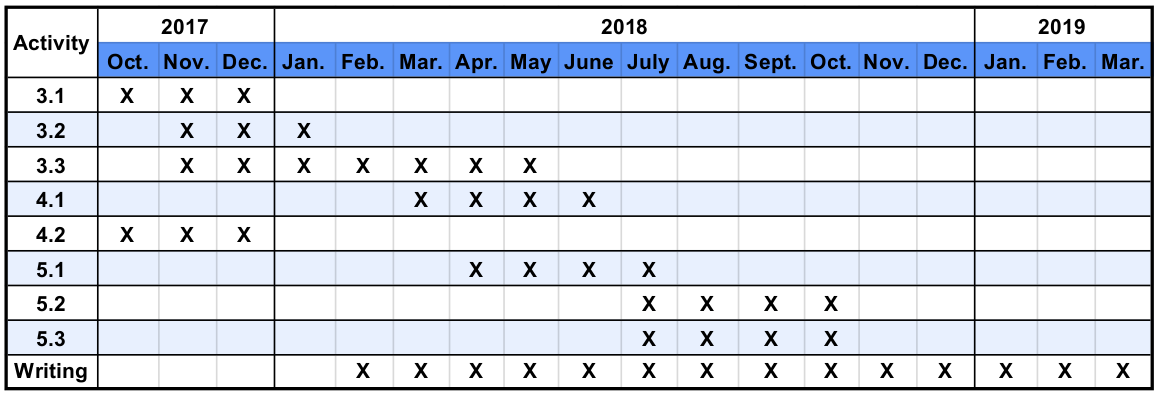
\includegraphics[scale=0.40]{images/Summary-Next-Steps.png}
		\caption{Schedule.}
		\label{fig:summary-next-steps}
	\end{center}
\end{figure}

We use, for example, 3.1 to denote the first item enumerated in the Research Status section of Chapter~\ref{sec:strategy} and so forth. 
The planned activities of the chapters not listed in Figure \ref{fig:summary-next-steps} are included in the writing activity.